\chapter{Beeintr�chtigung des Wohlbefindens}
\section{Multitasking}


Technische Ger�te wie Smartphones und Laptops sind ein fester Bestandteil der Gesellschaft geworden. Laut einer Studie \cite[p.~75]{Cyberkrank} besa�en im Jahr 2011 96\% von College-Studenten im Alter von 18 bis 22 Jahren ein Smartphone und 89\% Prozent der bereits Arbeitenden im gleichen Alter. In Deutschland gilt f�r die gleiche Altersgruppe �hnliches. 2011 besitzen in Deutschland 25\% ein Smartphone, 2013 sind es bereits 72\% Prozent \cite[p.~76]{Cyberkrank}. Dies ist nun 5 Jahre her. Es ist also plausibel, dass die �berwiegende Mehrheit heutzutage ein Smartphone besitzt.


Digitale Medien, welche rund um die Uhr �ber das Smartphone in der Tasche leicht zu erreichen sind, regen zum Multitasking an. Dabei ist es schwierig  f�r Menschen, Multitasking zu betreiben. Prof Dr. Torsten Schubert von der Humboldt\-Universit�t  behauptet, dass Multitasking durch Entscheidungsprozesse zu einer erh�hten Fehlerquote oder einer verl�ngerten Bearbeitungszeit \cite{Gehirn} f�hrt. Gem�� Schubert gilt generell: Wenn Aufgaben das gleiche Hirnareal beanspruchen, st�ren sie sich, wodurch Multitasking ineffizient wird. Die Natur des Menschen diktiert ihm sich vollst�ndig auf eine Aufgabe zu konzentrieren um diese zum Besten seiner F�higkeiten zu erledigen. Multitasking wird mit dem Antrainieren von Sucht und Aufmerksamkeitsst�rungen gleichgestellt \cite{Gehirn}.


Jugendliche nutzen ihr Smartphone im Schnitt 150 Mal am Tag. Folglich wird ihre T�tigkeit durchschnittlich alle 6 Minuten unterbrochen \cite[p.~28]{iDisorder}. Die Psychologin Lydia Burak von der Bridgewater State University f�hrte  eine Umfrage, \cite[p.~83]{Cyberkrank} (Massachusetts, USA) die bei einer Testgruppe von 774 Studenten im Alter von 20 bis 75 Jahren und einer Verteilung der Geschlechter von 67,1\% weiblich und 32,9\% m�nnlich mittels Fragebogen feststellt, dass sich nur 5,6\% nicht noch mit anderen Aktivit�ten w�hrend der Lehrveranstaltungen besch�ftigen. Dies ist interessant, da mithilfe eines Multiple-Choice Test kurz nach einer Vorlesung, die den darin behandelten Stoff abfragt, festgestellt werden konnte, dass die abgelenkten Studenten (Multitasking) schlechtere Resultate erzielten \cite[p.~87]{Cyberkrank}.

\begin{figure}
\centering
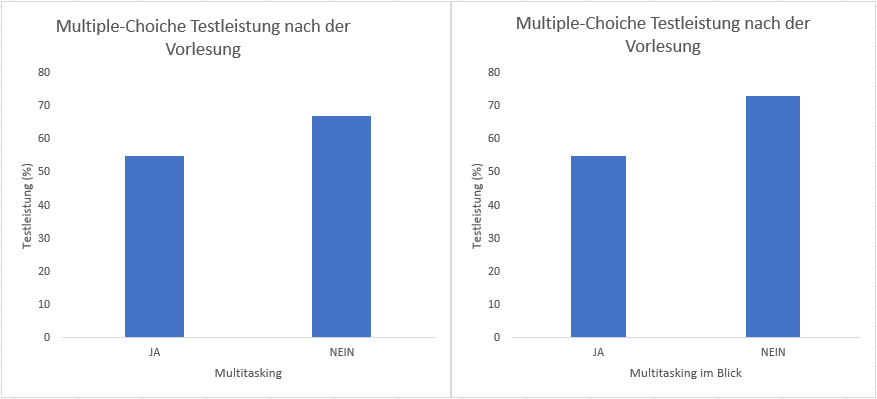
\includegraphics[scale=0.635]{images/graphtest.png}
\caption[Test ergebnisse von abgelenkten Studenten]{H�ufigkeit korrekter Antworten im Test nach der Vorlesung abh�ngig davon, ob die Studenten selbst gleichzeitig mit anderen Aufgaben am Computer besch�ftigt waren oder nicht (linke Abbildung) und abh�ngig davon, ob die Studenten anderen Studenten beim Multitasking am Laptop zuschauen konnten oder nicht (rechte Abbildung).}
\end{figure}


\section{Tr�bung der menschlichen Psyche}

Das Verwenden von Smartphones und Laptops st�rt das Lernen direkt durch Konzentrationsverlust w�hrend Lehrveranstaltungen und beeinflusst indirekt die akademische Leistung. Es wurde 2011 eine schwedische Studie von Biomedcentral Public Health \cite{Mobile} in Bezug auf die Relation zwischen Mobiltelefongebrauch und deren mentale Auswirkung durchgef�hrt.
Anhand 4156 Probanden, davon 1455 m�nnlich und 2701 weiblich, konnte eine Relation zwischen hohem Mobiltelefongebrauch, Stressempfinden, Schlafst�rungen und Symptomen von Depression festgestellt werden.
Die Probanden sind in einem Alter von 20 -24 Jahren von welchen 40\% der M�nner und 48\% der Frauen studieren.  Eine weiter Studie von Biomedcentral Psychiatrics \cite{Computer} von 2012 untersuchte bei 4163 Probanden im gleichen Alter, davon 1458 m�nnlich und 2705 weiblich, die gleichen Folgen bei hohem Computergebrauch.
Beide Studien verbinden die verbrachte Zeit in konstanter Erreichbarkeit durch Mobiletelefonen, und die Zeit vor dem Computer mit einem Risiko f�r erh�htes Stressempfinden, Schlafst�rungen oder Entwicklung von Symptomen der Depression.


Je mehr Zeit vor einem Bildschirm verbracht wird, desto gr��er ist der Einfluss auf die Art wie der Mensch mit seinem Sozialen Umfeld interagiert. Im Rahmen einer Studie aus Neuseeland \cite{Adolescent} wurden 1987\-1988 976 Jugendliche im Alter von 15 Jahren befragt, wieviel Zeit sie vor dem Fernseher verbringen und wie sie ihre Beziehung zu Gleichaltrigen und ihren Eltern mittels einer gek�rzten Version von \"Inventory of Parent and Peer Attachment\" (IPPA) bewerten. In der gleichen Studie wurden 2004 3983 Sch�ler aus 144 verschiedenen Schulen die gleichen Fragen gestellt. Anschlie�end wurden die Probanden gefragt, wieviel Zeit sie vor dem Computer verbringen und wieviel Zeit sie mit Lesen und dem Erledigen von Hausaufgaben in ihrer Freizeit verbringen.


In der ersten Phase 1987-1988 konnte  festegellt werden, dass jede weitere Stunde vor dem Fernseher das Risiko eine schlechte Beziehung mit den Eltern zu haben um 13\% erh�ht und mit Gleichaltrigen sogar um 24\%. In der zweiten Phase 2004 war das Resultat �hnlich, mehr Zeit vor dem Bildschirm egal ob Fernseher oder Computer f�hrte zu einem erh�hten Risiko eine schlechte Beziehung zu den Eltern oder Gleichaltrigen zu f�hren. Zeit mit Lesen und der Bew�ltigung von Hausaufgaben wurde hingegen mit einer besseren Beziehung zu den Eltern in Zusammenhang gebracht.